\documentclass{article}
\usepackage[utf8]{inputenc}
\usepackage[english]{babel}
\usepackage{amsthm}
\usepackage{amssymb}
\usepackage{mathcomp}
\usepackage{amsmath}
\usepackage{natbib}
\usepackage{array}
\usepackage{wrapfig}
\usepackage{multirow}
\usepackage{tabularx}
\usepackage{graphicx}
\usepackage{geometry}
\usepackage{multicol}
\usepackage{blindtext}


\title{Homework 4}
\author{Sean Eva}
\date{April 2022}

\begin{document}

\maketitle

\section{Theoretical Problems}
\begin{enumerate}
    \item [8.4: 3. ]
    
    \begin{center}
        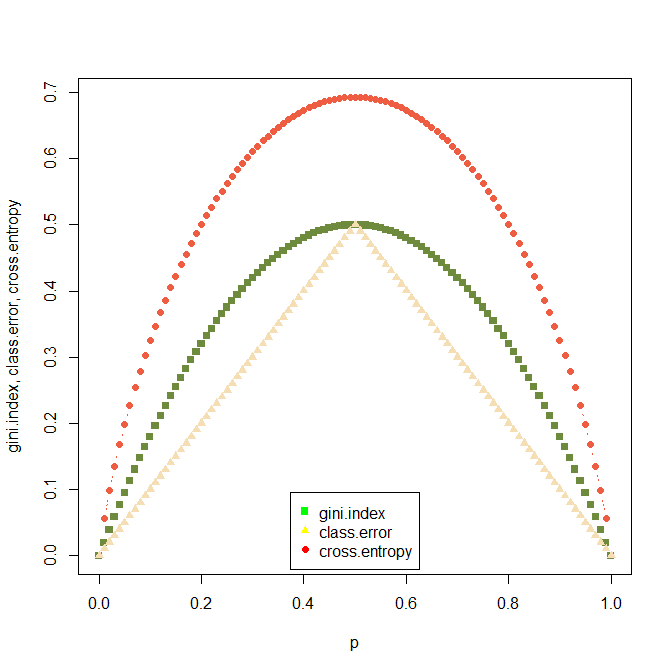
\includegraphics[width=7cm]{HW4_3.png}
    \end{center}
    
    \item [8.4: 4. ]
    
    \begin{enumerate}
        \item 
        
        \begin{center}
            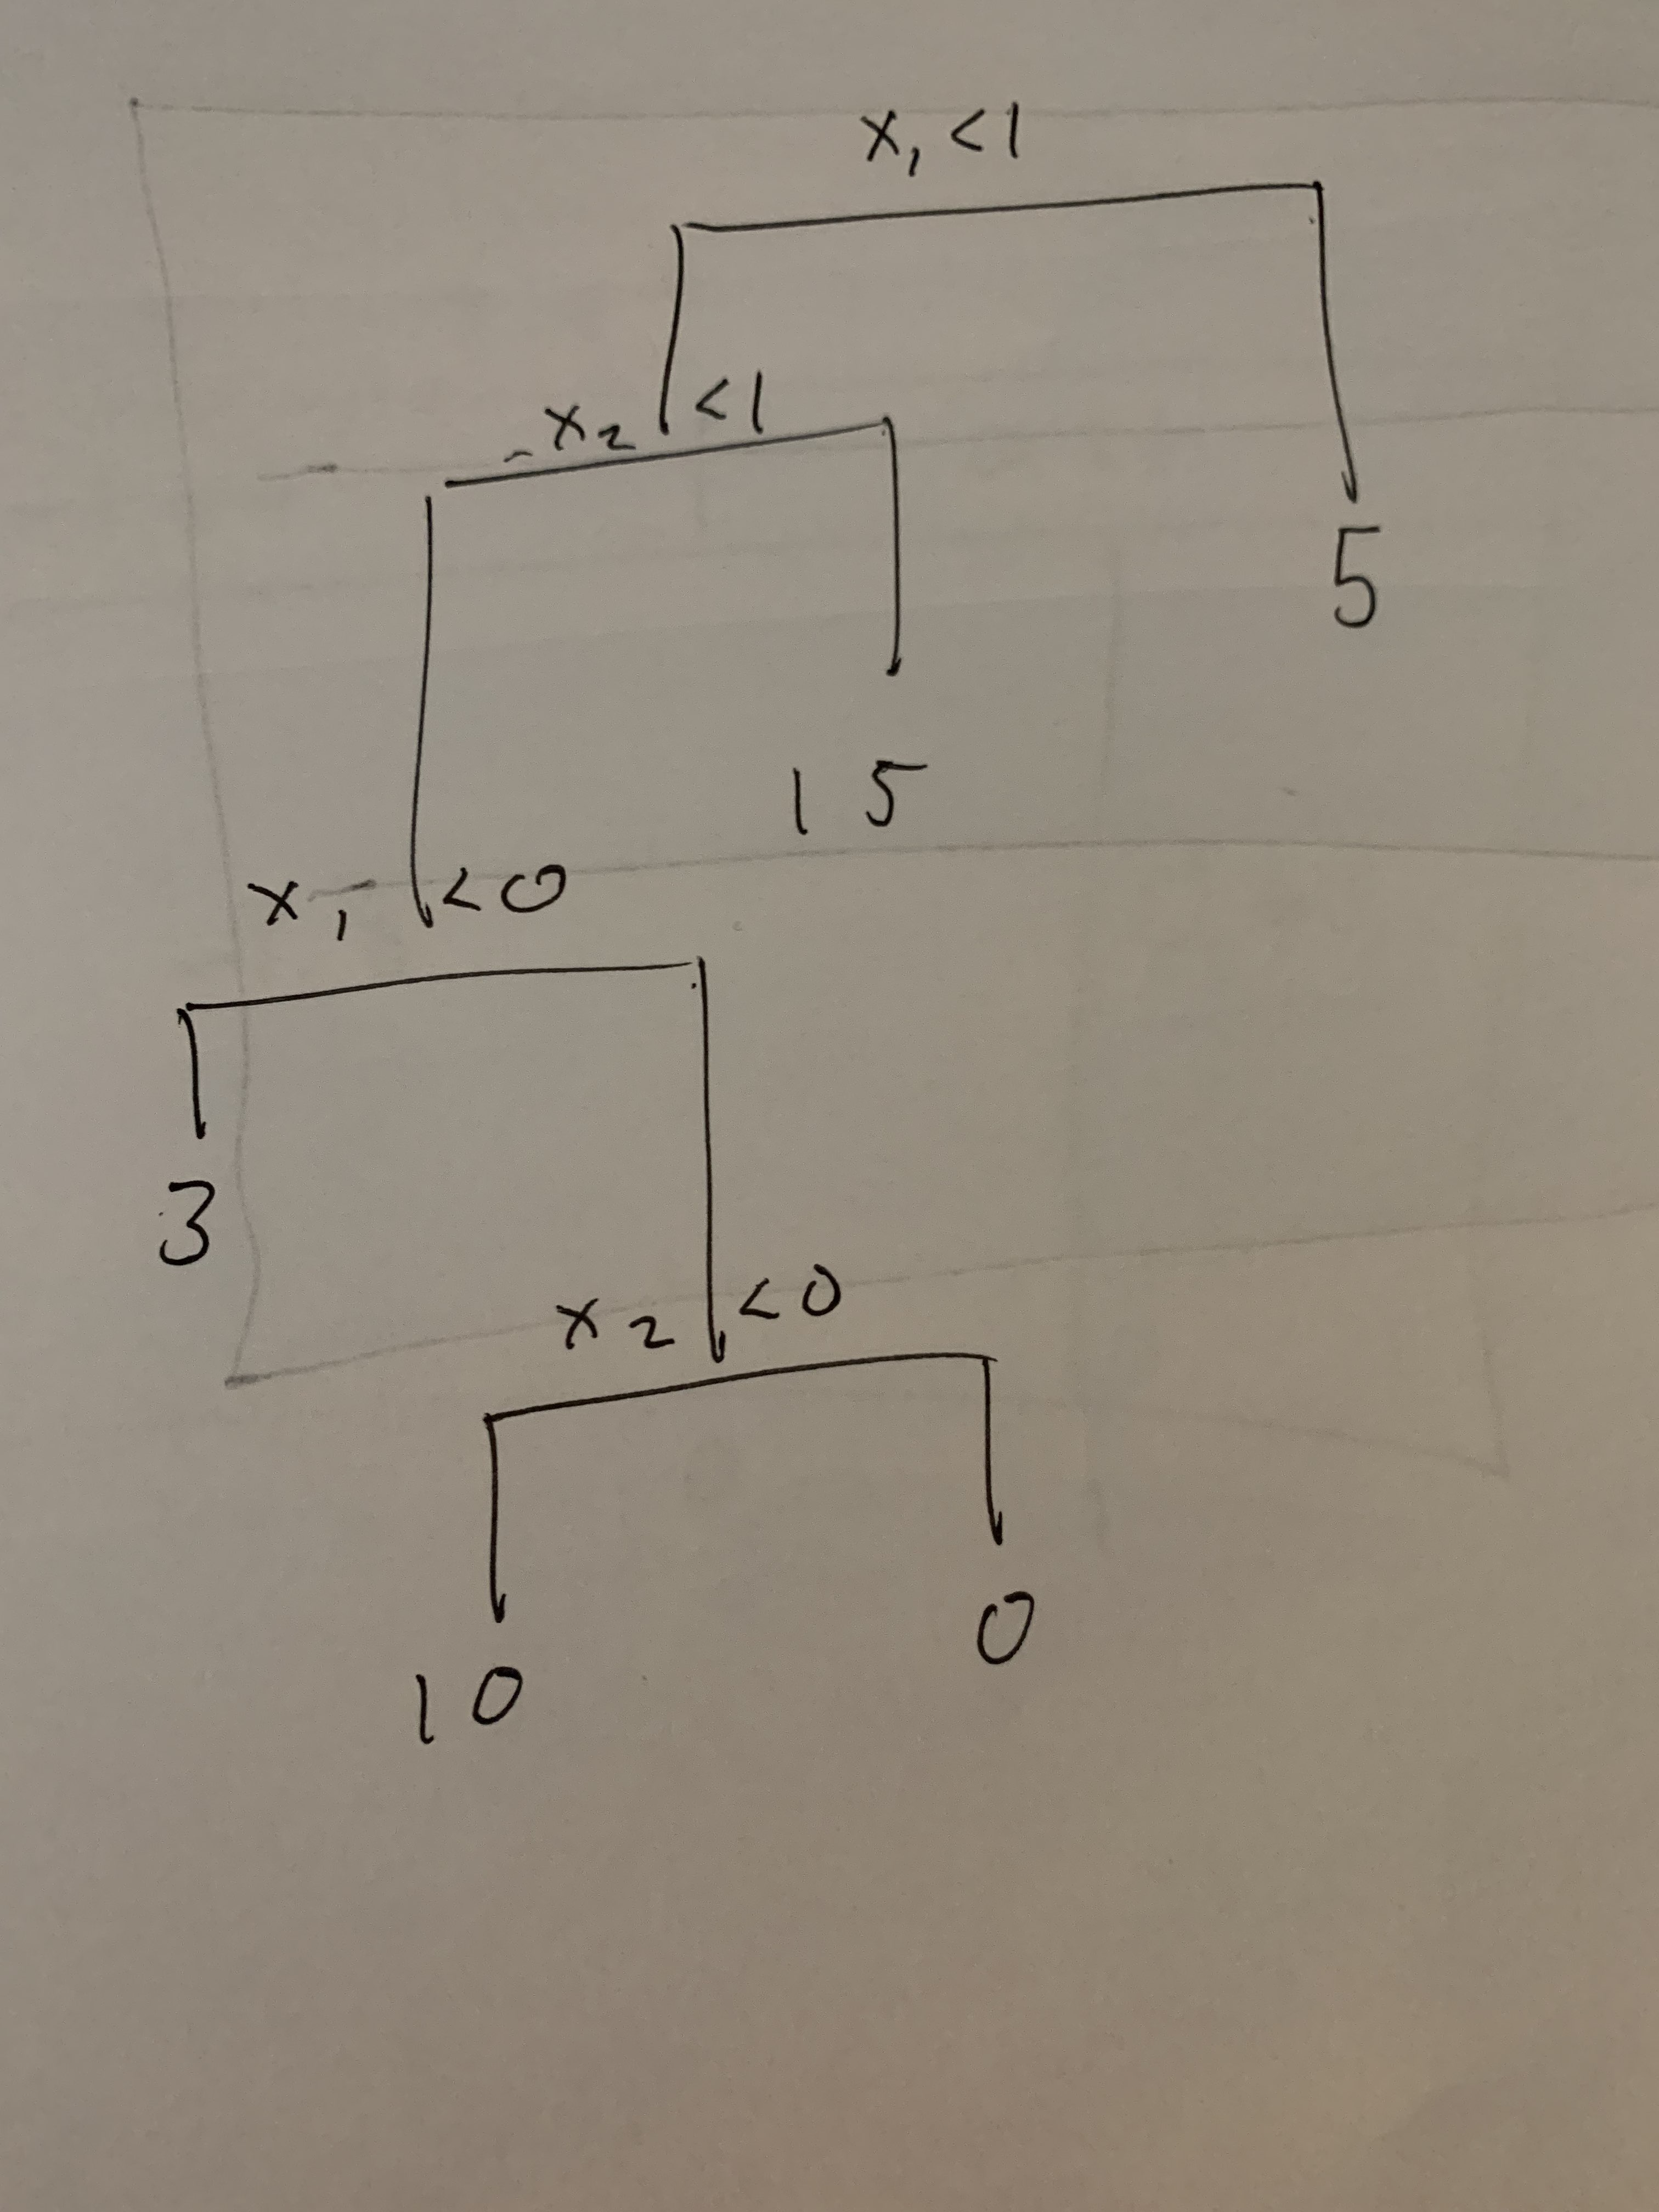
\includegraphics[width=5cm]{HW4_4a.jpg}
        \end{center}
        
        \item
        
        \begin{center}
            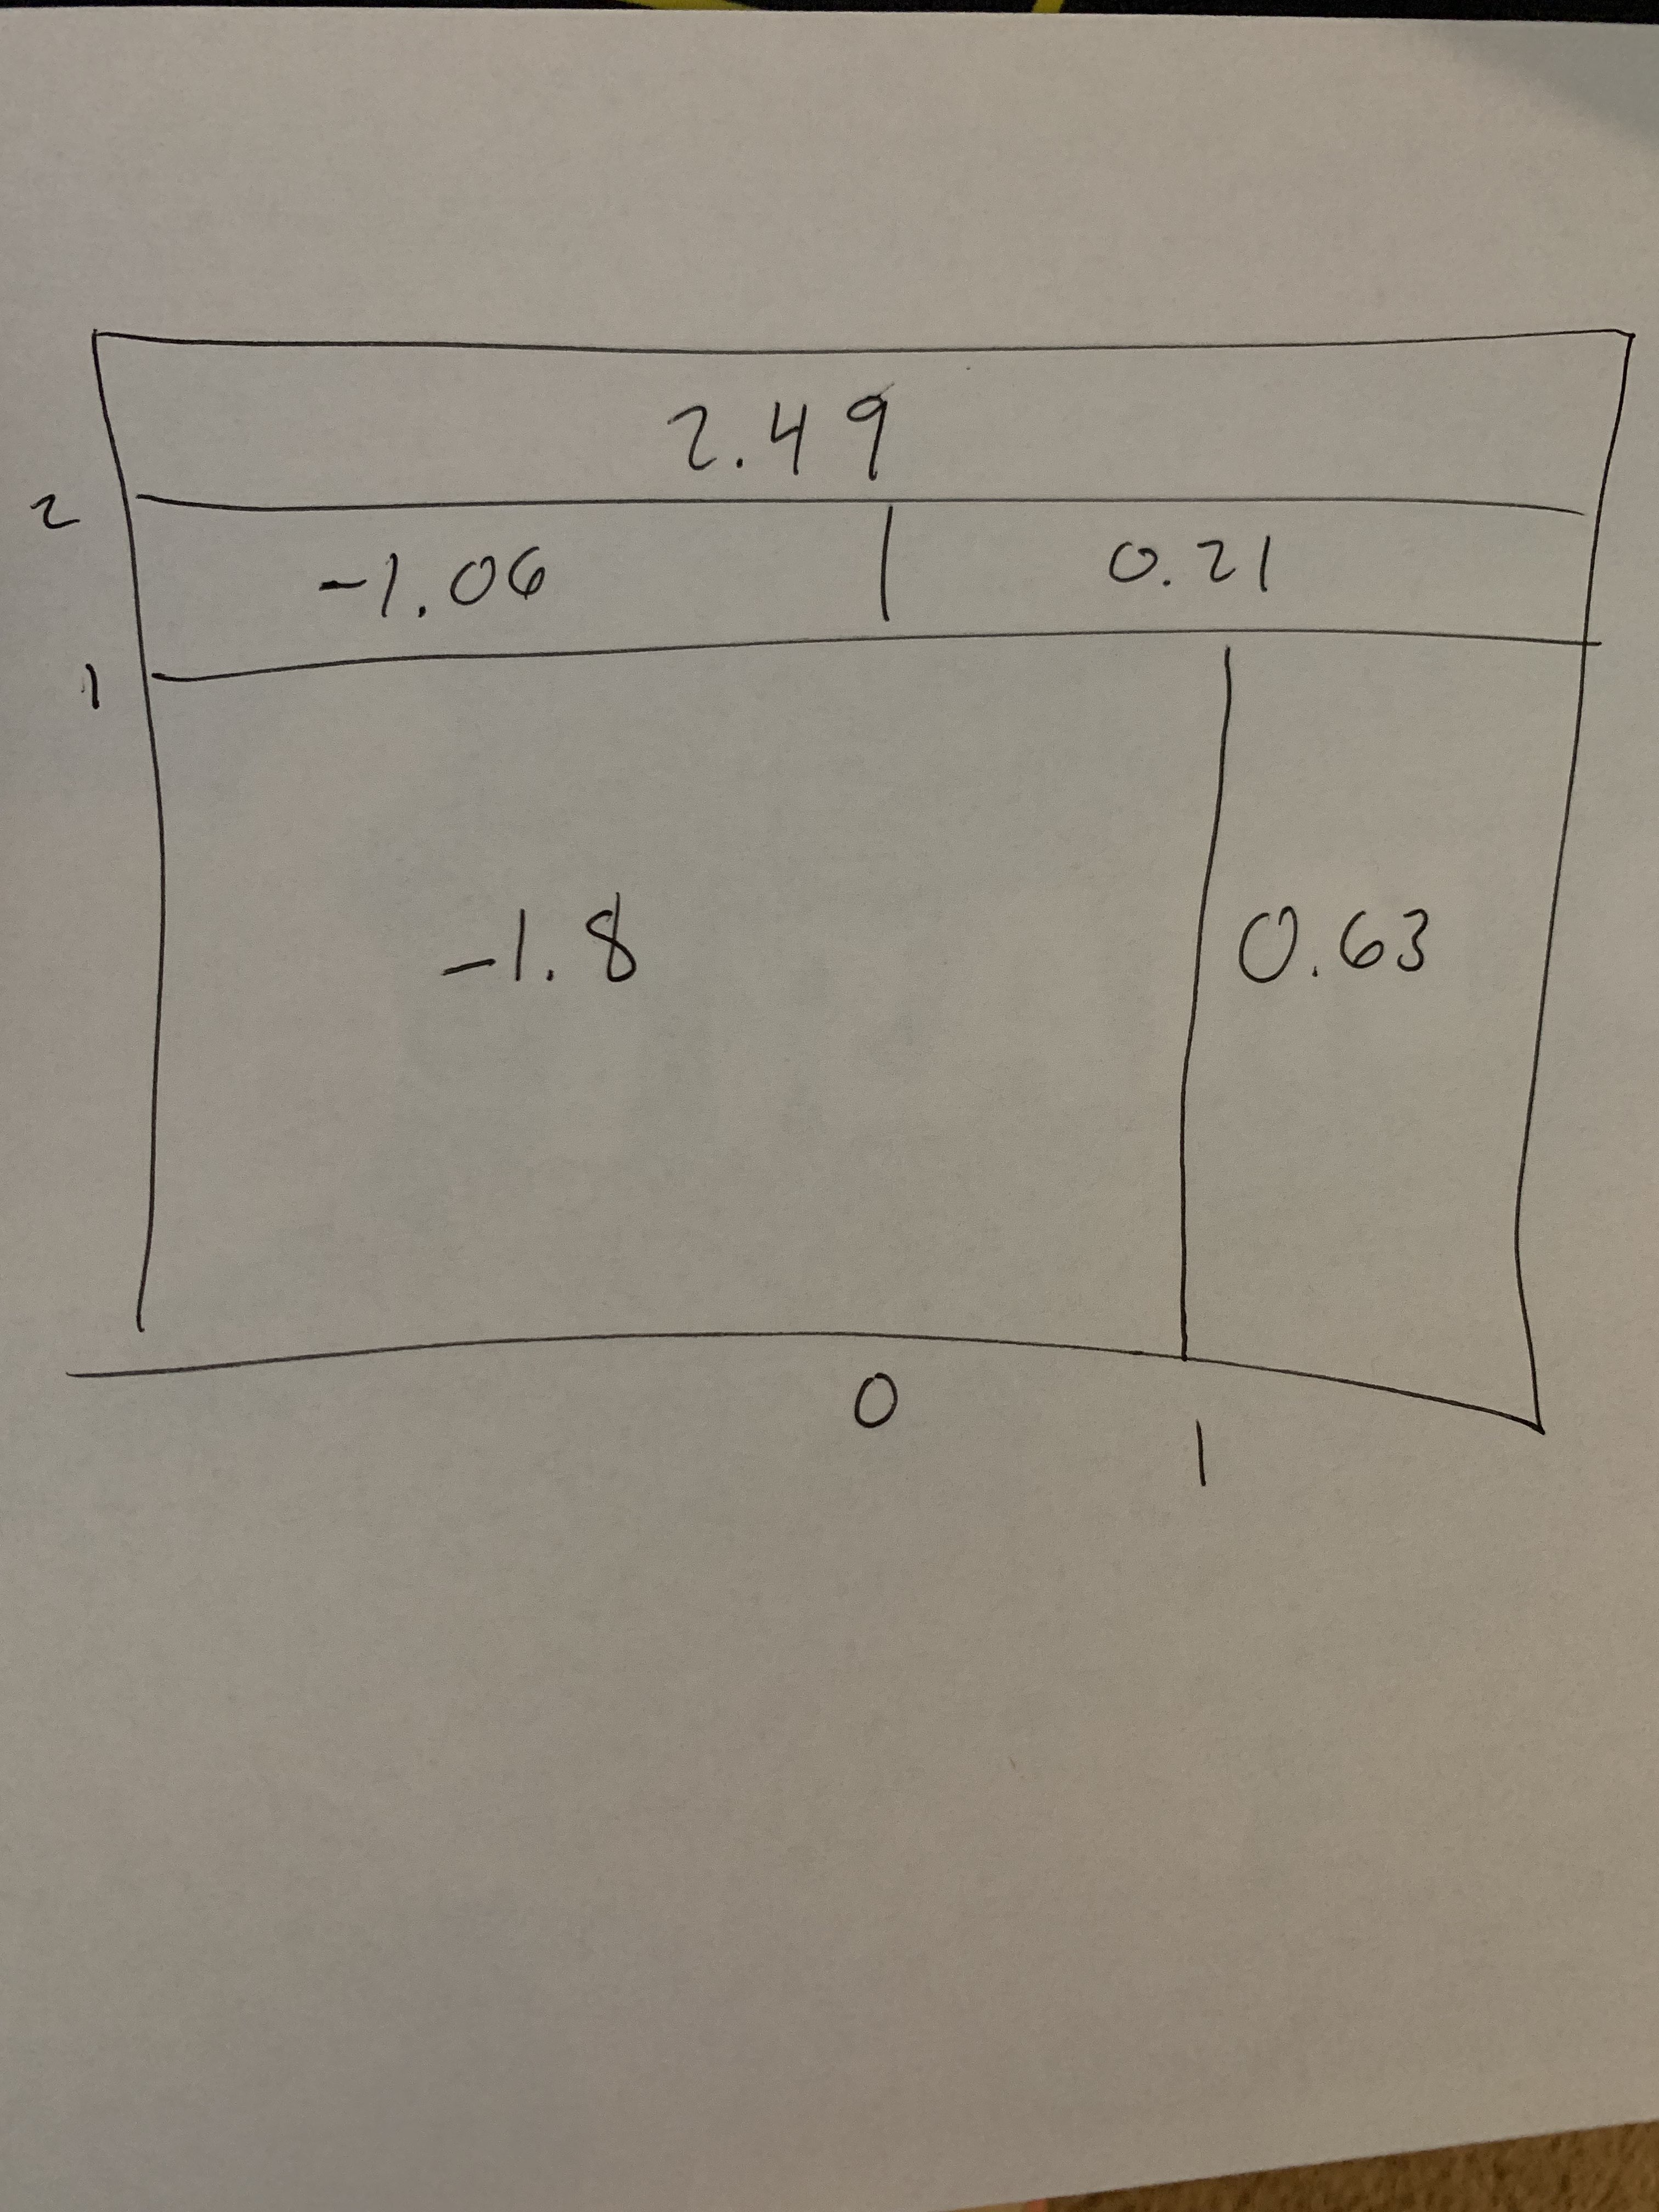
\includegraphics[width=5cm]{HW4_4b.jpg}
        \end{center}
        
    \end{enumerate}
    
    \item [8.4: 5. ]
    
    Using the majority vote method, we would find that there are 6 votes for red and only 4 votes for green which would lead us to conclude that the class if red. If we use an average probability method we would find an average $\mathbb{P}(\text{Class is Red}|X) = 0.45$ which would lead us to conclude that the class is green.
    
    \item [9.7: 2. ]
    
    \begin{enumerate}
        \item 
        
        \begin{center}
            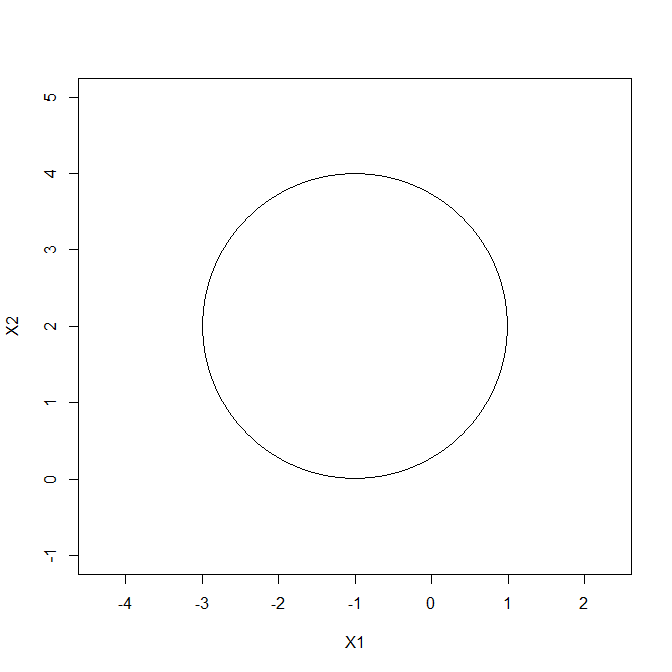
\includegraphics[width=8cm]{HW4_5a.png}
        \end{center}
        
        \item
        
        \begin{center}
            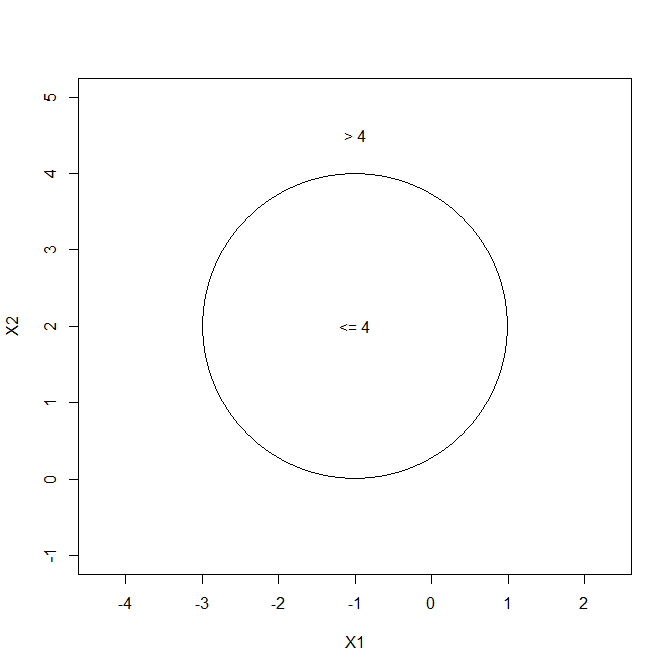
\includegraphics[width=8cm]{HW4_5b.png}
        \end{center}
        
        \item
        
        \begin{center}
            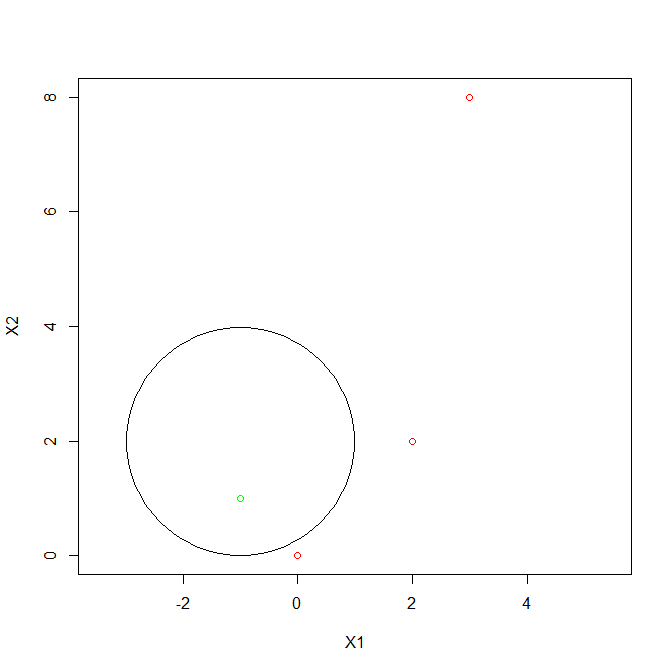
\includegraphics[width=8cm]{HW4_5c.png}
        \end{center}
        
        \item
        
        If we expand the equation of the decision boundary $(1 + X_1)^2 + (2 - X_2)^2 = 4$ which expands to $X_1^2 + X_2^2 + 2X_1 - 4X_2 + 1 = 0$ which is linear in terms of $X_1, X_1^2, X_2, \text{and} X_2^2.$
        
    \end{enumerate}
    
    \item [9.7: 3. ]
    
    \begin{enumerate}
        \item 
        
        \begin{center}
            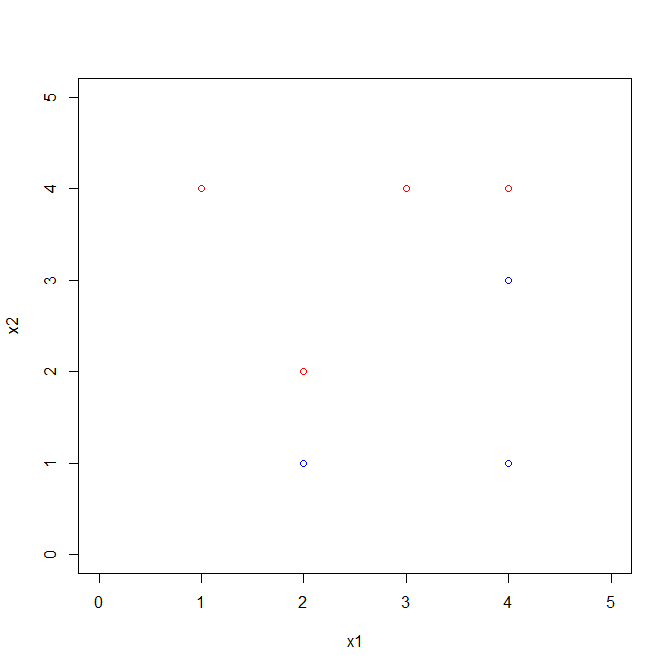
\includegraphics[width=8cm]{HW4_6a.png}
        \end{center}
        
        \item
        
        As shown in the plot, the optimal separating hyperplace has to be between the observations $(2, 1)$ and $(2, 2)$, and between the observations $(4, 3)$ and $(4, 4)$. So it is a line that passes through the points $(2, 1.5)$ and $(4, 3.5)$ which is the equation $X_1 - X_2 - 0.5 = 0.$
        \begin{center}
            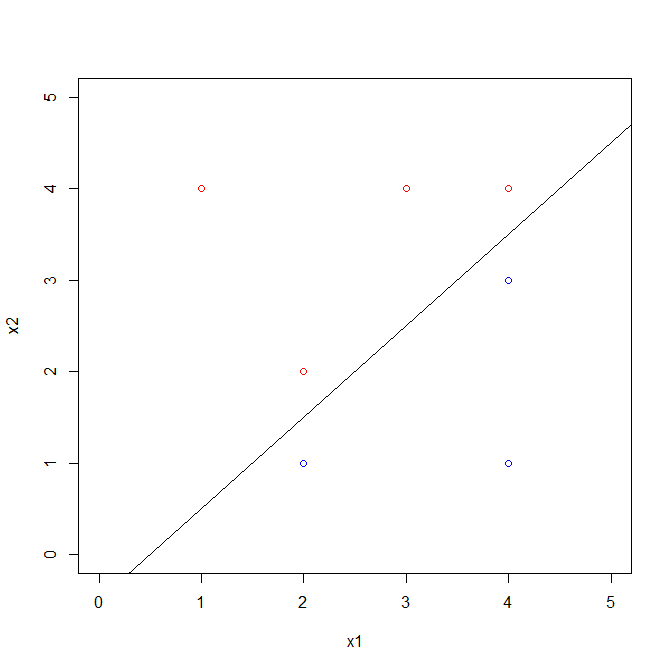
\includegraphics[width=8cm]{HW4_6b.png}
        \end{center}
        
        \item
        
        The classification rule is to classify as red if $X_1 - X_2 - 0.5 < 0$ and to classify as blue otherwise.
        
        \item
        
        \begin{center}
            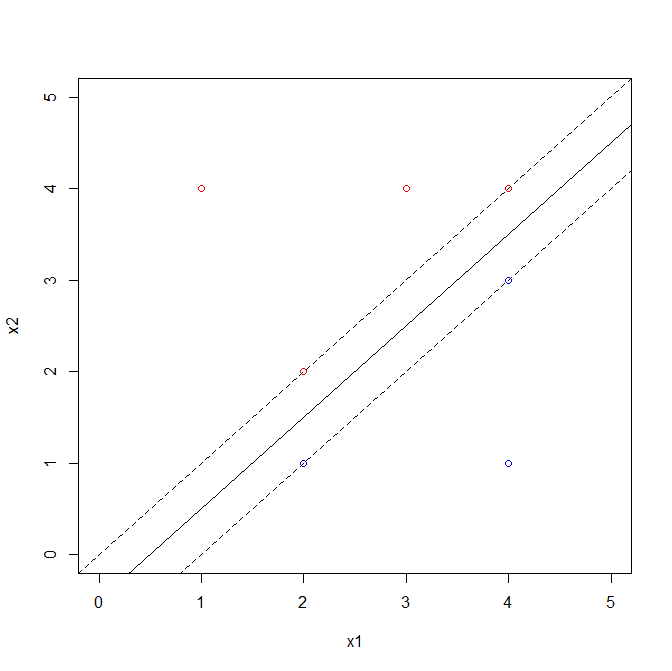
\includegraphics[width=8cm]{HW4_6d.png}
        \end{center}
        
        \item
        
        The support vectors are the points $(2, 1), (2, 2), (4, 3), $ and $(4, 4).$
        
        \item
        
        By examining the plot, it is easy to note that if we moved the observation $(4, 1)$, we would not change the maximal margin hyperplane because we did not classify it as a support vector.
        
        \item
        
        \begin{center}
            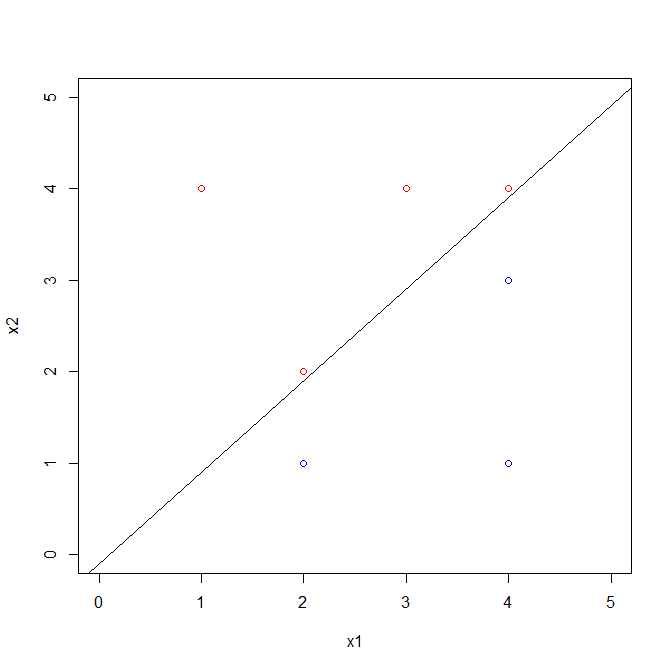
\includegraphics[width=8cm]{HW4_6g.png}
        \end{center}
        
        \item
        
        \begin{center}
            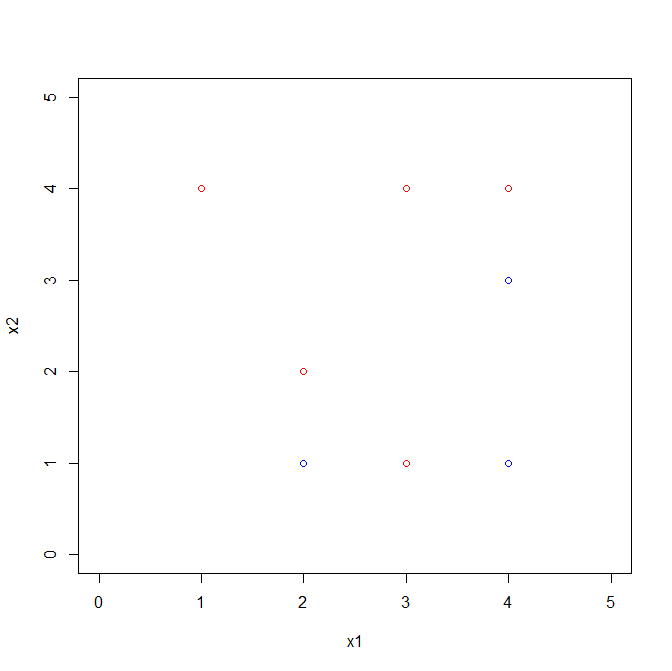
\includegraphics[width=8cm]{HW4_6h.png}
        \end{center}
        
    \end{enumerate}
    
\end{enumerate}
\section{Programming}
\begin{enumerate}
    \item [1. ]
    
    \begin{enumerate}
        \item 
        
        The test mean squared error 22.863431372549016
        
        \item
        
        When we performed this using $m=6 to m = 25$ we noticed the original tree expand. However, when we moved to $m = 100$ the tree did not grow a substantial amount.
        
        \item
        
        The error rate is about $19.2\%$.
        
        \item
        
        Sorry ran out of time.
        
    \end{enumerate}
    
    \item [2. ]
    
    \begin{enumerate}
        \item 
        
        In code.
        
        \item
        
        A cost of 1 seems to perform best.
        
        \item
        
        For a polynomial kernel, the lowest cross-validation error is obtained for a degree of 2 and a cost of 100. For a radial kernel, the lowest cross-validation error is obtained for a gamma of 0.01 and a cost of 100.
        
    \end{enumerate}
    
    \item [3. ]
    
    \begin{enumerate}
        \item 
        
        In code.
        
        \item
        
        Support vector classifier creates 435 support vectors out of 800 training points. Out of these 216 are in level MM and the other 219 are in CH.
        
        \item
        
        The training error is $17.5\%$ and the test error rate is about $17.8\%$.
        
        \item
        
        Optimal cost is 0.1.
        
        \item
        
        Training error rate is now $16.4\%$ and the test error rate is about $15.2\%.$
        
        \item
        
        Radial kernel with a default gamma creates 373 support vectors which 185 are in the MM level and the other 188 are in the CH level. The classifier has a training error of $15.1\%$ and a testing error of about $18.5\%$. Tuning does not reduce train and test error rates as we already used the optimal cost of 1.
        
        \item
        
        Polynomial kernel with default gamma creates 447 support vectors in which 225 are in the CH level and the other 222 are in the MM level. The classifier has a training error of $18.3\%$ and a testing error of about $22.2\%$. Tuning reduced train and test error rates.
        
        \item
        
        Overall, radial basis kernel seems to be producing the least misclassification error on both train and test data.
        
    \end{enumerate}
    
\end{enumerate}
\end{document}
